\documentclass[11pt,a4paper]{article}

\usepackage[T1]{fontenc}
\usepackage[utf8]{inputenc}
\usepackage[margin=2.5cm]{geometry}
\usepackage{mathptmx}
\usepackage[scaled=0.9]{helvet}
\usepackage{courier}
\usepackage{microtype}
\usepackage{amsmath}
\usepackage{booktabs}
\usepackage{tabularx}
\usepackage{array}
\usepackage{caption}
\usepackage{pgfplots}
\pgfplotsset{compat=1.18}
\usepackage[round,authoryear]{natbib}
\usepackage{xcolor}
\usepackage[hidelinks]{hyperref}
\usepackage{url}

\usepackage{needspace}
\usepackage{etoolbox}
% Layout: never leave a heading stranded at the bottom of a page.
% A section needs room for its heading plus about 8 lines of text,
% a subsection about 6 lines; otherwise it starts on the next page.
\pretocmd{\section}{\needspace{10\baselineskip}}{}{}
\pretocmd{\subsection}{\needspace{7\baselineskip}}{}{}
% No single first/last lines of a paragraph alone on a page.
\clubpenalty=10000
\widowpenalty=10000
\displaywidowpenalty=10000
% Let pages end short instead of stretching the vertical space.
\raggedbottom
% Allow floats to take more of a page, so tables stay near their text.
\renewcommand{\topfraction}{0.85}
\renewcommand{\textfraction}{0.15}
\renewcommand{\floatpagefraction}{0.75}
\newcommand{\x}{\ensuremath{\times}}
\newcolumntype{L}{>{\raggedright\arraybackslash}X}
\definecolor{accent}{RGB}{38,110,210}
\definecolor{muted}{RGB}{190,190,180}

\title{The Byte Tax: Decode Speed of Byte-Level Language Models on a Consumer GPU}
\author{Fabio-Eric Rempel\\[2pt]
  \small Independent researcher, Detmold, Germany\\
  \small ORCID \href{https://orcid.org/0009-0008-8447-6159}{0009-0008-8447-6159}}
\date{November 2026}

\begin{document}
\maketitle

\begin{abstract}
Byte-level language models remove the tokenizer, but at batch size~1 they decode more slowly per generated byte than the token model they come from. We measure this \emph{byte tax} for Bolmo~1B, a byteified OLMo~2~1B, against its source on a consumer GPU (RTX~3060~Ti), through a chain of 67~hypotheses written down before each measurement. In eager decoding Bolmo is 2.36\x{} slower per byte. Most of the gap is launch and host overhead in its per-byte local encoder and decoder: CUDA graphs and a single-sync decode loop make Bolmo 3.8\x{} faster, byte-identically, and leave a gap of 1.5\x{} that follows a memory-bandwidth model. Weight quantization confirms the model and shows that the per-byte local stack is the cheapest part to quantize, saving 4.1\x{} more time per gigabyte than the global transformer. Speculative drafting first widens the tax to 2.37\x: a token model verifies several drafted tokens almost for free, and a byte model's drafting rounds end and restart at byte granularity. Aligning drafting rounds to patch boundaries reverses this. It makes Bolmo 2.06\x{} faster than its plain loop in bf16, exact in fp32, and narrows the drafted tax to 1.36\x, below the undrafted 1.49\x. Optimizations of weight reads favour the token model, and at int8 the tax settles at 1.60\x, about 13\% above the bandwidth floor for that configuration. A kernel census and microbenchmarks show that the remaining overhead is kernel count, not synchronization, and that a persistent megakernel would gain only 4 to 8\%. Overall Bolmo becomes 10.3\x{} faster than eager, and 26 of the 67~hypotheses were refuted.
\end{abstract}

\section{Introduction}

The speed gap between byte-level and token-level models at batch size~1 is not fixed: it depends on which optimizations are applied, and most standard optimizations favour the token model.

Byte-level models read raw UTF-8 bytes instead of subword tokens. They avoid tokenizer artifacts, handle character-level tasks better, and treat all languages and scripts alike, and recent scaling studies find they can reach a higher quality ceiling than token models \citep{marathe2026tokenceiling,wang2026bytelm}. Their main cost has been efficiency: a text has about four times as many bytes as tokens. Latent-tokenizer architectures \citep{pagnoni2025blt,hwang2026hnet} answer this by grouping bytes into patches, so a large global transformer runs once per patch while small local layers run once per byte. Byteification \citep{minixhofer2026byteification} converts an existing subword model into such an architecture with under 1\% of a pretraining budget, which for the first time gives a byte model and a token model that share the same global transformer and training lineage.

That pairing makes a clean measurement possible. We compare Bolmo~1B with OLMo~2~1B, the model it was byteified from, at batch size~1 on a consumer GPU, the setting of local, single-user inference.

\needspace{8\baselineskip}
\noindent We ask:
\begin{enumerate}
  \item Where does decode time go in the byte model, compared with its source?
  \item How much of the gap is overhead that standard techniques remove?
  \item Does the remaining gap follow a memory-bandwidth model, and which part of the byte model carries it?
  \item Does speculative drafting close the gap or widen it, and why?
  \item How close does the byte model get to the hardware floor?
\end{enumerate}
Every step was a written study with hypotheses fixed before measurement; 26 of 67 were refuted, including several of our own explanations, and all are reported in a companion technical report.

\paragraph{Contributions.}
\begin{itemize}
  \item A decomposition of the byte tax into launch overhead, weight bandwidth and per-kernel cost, validated by intervention rather than profiling alone.
  \item The finding that the per-byte local stack is the most efficient place to quantize a byte model.
  \item A mechanism for why speculative drafting favours coarse units: the free unit per round and the restart position after a miss.
  \item Boundary-gated drafting, which aligns rounds to patches and turns drafting from widening the byte tax (2.37\x) into narrowing it (1.36\x).
  \item A bandwidth-floor analysis showing the remaining tax at int8 is within about 13\% of what this hardware allows.
\end{itemize}

\section{Background and setup}

Bolmo and OLMo~2 share their 16-layer global transformer; the byte model adds a small local stack that runs on every byte.

\subsection{The models}

Bolmo~1B (\texttt{allenai/Bolmo-1B}, revision \texttt{452690a8}) has four parts. A local encoder (one mLSTM layer \citep{beck2025xlstm} with an MLP) contextualizes each byte. A boundary predictor decides where patches end during prefill; during decoding the boundary flag is part of the output, using a fused vocabulary of 256~bytes plus 256 byte-with-boundary atoms. The global model, OLMo~2's 16~transformer layers, runs once per patch. A local decoder (four mLSTM layers) turns the patch representation back into byte predictions. Patches average 3.4 to 3.8~bytes, close to a token. OLMo~2~1B (\texttt{allenai/OLMo-2-0425-1B}; \citealp{walsh2025olmo2}) runs its full model once per token, including a 100k-entry output head of about 0.21B parameters, about the size of Bolmo's local stack (about 0.18B).

\subsection{Hardware and workload}

All headline numbers come from one RTX~3060~Ti (8~GB, Windows, measured copy bandwidth 411~GB/s), batch size~1, greedy decoding and a fixed seed. Timing uses five prompts (English, Python, German, JSON, mixed Unicode) with 256 new bytes; OLMo generates 72~tokens (about 259~bytes) so cache sizes match. Drafting parameters were tuned on a separate set of 25~prompts. A Linux Tesla~T4 run in fp32 served as a cross-check of the eager ratio (2.09\x{} against 2.25\x{} on Windows).

\subsection{Measurement}

A small harness hooks each component with CUDA events and also runs every workload without hooks for true throughput (hooks add 5 to 7\%). The metric is milliseconds per generated UTF-8 byte. Quality is measured as bits per byte on the first 200{,}000 bytes of WikiText-2 test and as accuracy on 1{,}500 items of CUTE \citep{edman2024cute}, a character-manipulation benchmark. Optimized outputs are compared byte for byte with eager output; in fp32 all drafted and graphed variants are identical, while bf16 runs diverge only at near-ties of the top two logits.

\subsection{Protocol}

Each of the 13 hypothesis-driven studies was a written task with hypotheses and the author's predictions copied verbatim into a findings file before any measurement and never edited afterwards. Every speed cell was run twice; pairs differing by more than 5\% were rerun. Most studies ended with a cost-model gate: a variant was built only if its predicted gain cleared a threshold set in advance. Experiments were run by Claude Code under these written specifications.

\section{Where the time goes}

In eager decoding the byte tax is the per-byte local loop, and most of that loop is overhead rather than computation.

\subsection{Eager profile}

In eager Hugging Face decoding, Bolmo needs 15.0~ms per byte and OLMo~2 6.36~ms (2.36\x). The global transformer costs almost the same per byte in both models (about 6.8 against 6.4~ms), because a 3.4-byte patch compresses nearly as well as a 3.6-byte token. The gap is Bolmo's local encoder and decoder: about 9~ms per byte, against 0.7~ms for OLMo's embedding, norm and head. A global layer costs about 1.4~ms per call in both models, roughly 4.4\x{} what its weight reads require. On a Linux T4 trace the GPU was busy 35.5\% of the time during Bolmo generation and 63.8\% during OLMo generation, with about 430 and 220 kernels per byte.

\subsection{Removing overhead}

\begin{table}[htbp]
\centering
\caption{Overhead removal for Bolmo~1B, bf16, default prompts, 256 new bytes.}
\label{tab:overhead}
\begin{tabular}{lrr}
\toprule
Variant & ms/byte & Speedup vs eager \\
\midrule
Eager & 15.01 & 1.00\x \\
CUDA graph, local loop & 8.76 & 1.71\x \\
CUDA graph, local loop and global model & 4.85 & 3.09\x \\
Single-sync decode loop & 3.97 & 3.78\x \\
\bottomrule
\end{tabular}
\end{table}

Capturing the decode step in CUDA graphs removes per-kernel launch work from the CPU; output stays byte-identical to eager (Table~\ref{tab:overhead}). The remaining host loop made nine syncs per byte. A replacement loop with one sync per byte, which reads the generated byte and its boundary flag in one copy and computes subword-suffix ids with an Aho--Corasick automaton (exact against the tokenizer on about 30{,}000 positions), removes it. Contrary to our prediction, the host loop was only 21\% of the graphed time; the $O(n)$ history walk we suspected cost 47~$\mu$s per call. With the same loop treatment, OLMo~2 reaches 2.58~ms/byte, so the gap is 1.54\x.

\subsection{The bandwidth model}

Once overhead is gone, decoding is bound by weight reads. Bolmo reads about 1.0~GB of weights per output byte in bf16: 0.64~GB for the global model, read once per patch, and 0.36~GB for the local stack, read on every byte. OLMo~2 reads about 0.75~GB. A fit of
\begin{equation}
  t_{\text{byte}} = t_{\text{fixed}} + k \cdot W_{\text{byte}},
\end{equation}
where $W_{\text{byte}}$ is weight bytes read per output byte, reproduces five quantized variants within about 2\%, with $t_{\text{fixed}} \approx 1.15$~ms per byte. Quantization savings arrive at a steady 71 to 77\% of the model's prediction; the shortfall is that fixed part, which later turned out to be per-kernel cost (Section~\ref{sec:floor}).

\section{Quantization: the cheapest place is the per-byte stack}

Because local weights are read once per byte and global weights once per patch, quantizing the local stack saves the most time per gigabyte and costs the least quality per millisecond.

\begin{table}[htbp]
\centering
\caption{Weight-only round-to-nearest quantization of Bolmo~1B on the graphed single-sync loop. bpb: bits per byte on WikiText-2; CUTE change in points.}
\label{tab:quant}
\begin{tabular}{lrrr}
\toprule
Variant & ms/byte & bpb change & CUTE change \\
\midrule
bf16 & 3.978 & 0 & 0 \\
Local int8 & 3.422 & +0.08\% & +0.2 \\
Global int8 & 3.175 & +0.00\% & $-0.2$ \\
Local int4 & 3.132 & +1.2\% & $-2.2$ \\
Local int4 + global int8 & 2.492 & +1.2\% & $-2.4$ \\
Global int4 & 2.729 & +3.5\% & $-4.2$ \\
All int4 & 1.992 & +4.9\% & $-6.2$ \\
\bottomrule
\end{tabular}
\end{table}

Per gigabyte of weights quantized, local layers save 4.06\x{} more time than global layers, close to the 3.4\x{} expected from bytes per patch (Table~\ref{tab:quant}). Per millisecond saved, local int4 costs 1.4\% bits per byte and global int4 2.8\%. The int8 tier is essentially lossless, as for token models; local int4 with plain rounding costs about what calibrated int4 methods cost a 7B token model on WikiText-2 (+1.5 to 1.6\% in cross-entropy from GPTQ and AWQ results reported by \citealp{shao2024omniquant}). Calibrated quantization of the full model was not tested.

A fair comparison needs the same kernels, loop and precision rule for both models. With each model at its best precision, the ratio is 1.49\x{} (bf16), 1.40\x{} (int8) and 1.48\x{} (int4). Under a rule that keeps output heads in bf16, the int4 ratio drops to 1.12\x, because OLMo's 421~MB head stays expensive while Bolmo's 520-entry head is tiny: a real structural advantage of byte models, but not an even contest.

\section{Why speculative drafting favours coarse units}

Naive drafting makes the byte model faster but the token model much faster, because a token model verifies drafts almost for free and a byte model's rounds end and restart at byte granularity.

\subsection{Drafting within patches}

In speculative decoding \citep{leviathan2023speculative,chen2023speculative} a cheap drafter proposes $K$ units and the target model verifies them in one pass; greedy verification keeps the output exact. Our drafter is a lookup drafter: it copies a continuation from earlier context (prompt-lookup style; \citealp{saxena2023promptlookup}), otherwise uses a byte $n$-gram table built from 19.4~MB of text with no 32-byte overlap with any prompt. For Bolmo, a round verifies the drafted bytes with the local encoder and decoder in one CUDA graph and stops at the first patch boundary, because the global model must run before the next patch. It emits 2.0 to 2.3 bytes per round and makes Bolmo 1.19\x{} faster in bf16 (3.995 to 3.361~ms/byte), with fp32 output identical in all 240 runs. The same drafter family on token ids makes OLMo~2 1.89\x{} faster (2.688 to 1.420), so the ratio grows from 1.49\x{} to 2.37\x.

\subsection{The verification asymmetry}

At batch~1, a forward pass reads every weight once whether it processes one position or nine, and the GPU's compute is mostly idle; OLMo verifies 9~tokens for 8\% more than~1. Bolmo can batch only its local stack, about 37 to 40\% of its time, while the global model still runs once per patch. Its mLSTM recurrence also steps through drafted positions in sequence, and small matrix multiplications with 2 to 9 rows hit a gap in standard kernels: cuBLAS switches from gemv to padded $64\times64$-tile gemm, so one gate projection goes from 3.5 to 10.8~$\mu$s. A fused multi-step recurrence kernel cut the recurrence from 16.1 to 4.5~$\mu$s per extra position, but gained only about 1\% end to end.

\subsection{Free unit and restart position}

The same small-model drafter continuations give OLMo~2 about 2.7\x{} the bytes per round that they give Bolmo. A protocol audit and a two-by-two comparison (each model's text under each model's acceptance rule) locate the cause in the round protocol, not the text (Table~\ref{tab:factors}).

\begin{table}[htbp]
\centering
\caption{Decomposition of the acceptance gap, SmolLM2-360M drafter.}
\label{tab:factors}
\begin{tabular}{lr}
\toprule
Factor & OLMo vs Bolmo, bytes per round \\
\midrule
Text predictability & 0.89\x \\
Boundary flags must match (Bolmo only) & 1.05\x \\
Free unit per round and restart position & 2.6\x \\
Byte vs token matching & 1.1\x \\
\bottomrule
\end{tabular}
\end{table}

Every round ends with one unit the target predicts itself: a token of about 4~bytes for OLMo, one byte for Bolmo. And 68\% of Bolmo's rounds then restart inside a token, where a token-level drafter's first guess is right 17 to 23\% of the time, against 77 to 86\% elsewhere. Granularity explains only part of that: rounds restart where the drafter has just missed, and misses cluster at hard positions, which in a byte model fall mid-token. This is the tokenization bias described by \citet{phan2025exact} appearing inside speculative decoding. By the chain rule a byte model does not make more hard guesses than a token model; it makes more steps, and its drafting rounds are cut at byte granularity.

\section{Patch-aligned drafting}

Gating cross-patch drafts to rounds that start at a patch boundary makes Bolmo 2.06\x{} faster than its plain loop in bf16 and brings the drafted byte tax below its undrafted level.

\begin{figure}[!b]
\centering
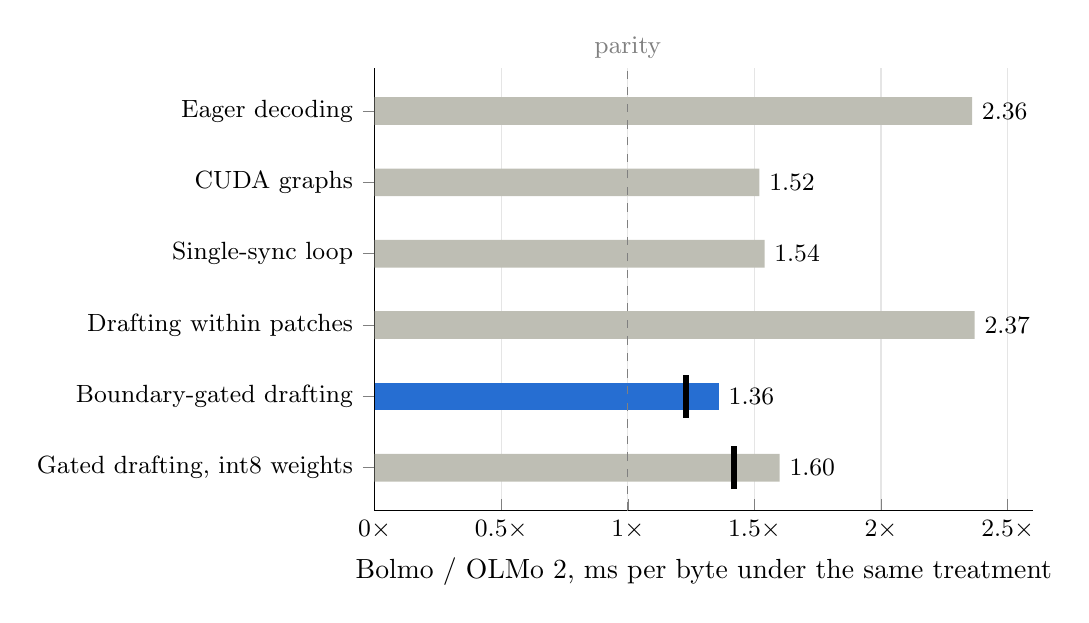
\begin{tikzpicture}
\begin{axis}[
  xbar,
  bar shift=0pt,
  width=0.82\textwidth,
  height=7.2cm,
  bar width=10pt,
  xmin=0, xmax=2.6,
  ymin=0.4, ymax=6.6,
  xlabel={Bolmo / OLMo~2, ms per byte under the same treatment},
  ytick={1,2,3,4,5,6},
  yticklabels={
    {Gated drafting, int8 weights},
    {Boundary-gated drafting},
    {Drafting within patches},
    {Single-sync loop},
    {CUDA graphs},
    {Eager decoding}},
  y tick label style={font=\small},
  x tick label style={font=\small},
  xtick={0,0.5,1,1.5,2,2.5},
  xticklabel={\pgfmathprintnumber[fixed,precision=1]{\tick}\x},
  nodes near coords,
  nodes near coords style={font=\small},
  point meta=x,
  every node near coord/.append style={/pgf/number format/fixed,/pgf/number format/fixed zerofill,/pgf/number format/precision=2},
  axis x line*=bottom,
  axis y line*=left,
  xmajorgrids=true,
  grid style={gray!20},
  clip=false,
]
\addplot[fill=muted, draw=none] coordinates {
  (1.60,1) (2.37,3) (1.54,4) (1.52,5) (2.36,6)};
\addplot[fill=accent, draw=none] coordinates {(1.36,2)};
\draw[dashed, gray] (axis cs:1,0.4) -- (axis cs:1,6.6)
  node[above, font=\small, text=gray] {parity};
\draw[line width=2.2pt] (axis cs:1.23,1.7) -- (axis cs:1.23,2.3);
\draw[line width=2.2pt] (axis cs:1.42,0.7) -- (axis cs:1.42,1.3);
\end{axis}
\end{tikzpicture}
\caption{The byte tax across optimization stages. Generic steps leave the ratio near 1.5\x{} or widen it; boundary-gated drafting is the only step that moves it toward parity. Black ticks mark the ratio if both models ran at their weight-bandwidth floor (Section~\ref{sec:floor}). Last row: int8 global weights for Bolmo, int8 blocks for OLMo~2, skinny kernels for both. bf16 unless noted.}
\label{fig:ratio}
\end{figure}

\subsection{Design}

Drafts that cross patch boundaries would batch the global model too: one global pass over eight patches costs only 1.08\x{} a pass over one (7.69 to 8.33~ms in bf16). Crossing in every round gains little, though, because each round then pays a speculative global pass that is lost when the draft is rejected. Small token-model drafters (SmolLM2-135M and -360M, Qwen2.5-0.5B) do not fix this: they emit at most 4.5 bytes per round and cost 3.7 to 5.5~ms per drafted token, more than a whole Bolmo round. Bolmo's boundary flags, however, follow the OLMo~2 tokenizer's segmentation of its own output on 98.7\% of byte positions, so a lookup draft can be given flags by re-tokenizing it.

Boundary-gated drafting uses two kinds of round. A round that starts mid-patch drafts only to the end of the current patch with the lookup drafter, with no global pass. A round that starts at a boundary drafts across patches, takes flags from re-tokenization, and runs one global pass over all speculative patches. Acceptance requires both byte and flag to match; rollback restores the recurrent states and the global cache position.

\subsection{Results}

\begin{table}[htbp]
\centering
\caption{Boundary-gated drafting, default prompts, ms per generated byte.}
\label{tab:gated}
\begin{tabular}{lrrrr}
\toprule
Precision & Plain loop & Within-patch & Boundary-gated & Gain over within-patch \\
\midrule
bf16 & 3.975 & 2.798 & 1.934 & +30.9\% \\
all-int4 & 1.998 & 1.686 & 1.456 & +13.6\% \\
\bottomrule
\end{tabular}
\end{table}

Bytes per global pass rise from about 3.8 to 7.2, matching the simulation exactly on the tuning prompts (Table~\ref{tab:gated}). A crossing round costs at most 0.10~ms beyond the pieces the cost model already contained, and the model predicted the bf16 and int4 results within 12.6\% and 0.1\%. In bf16, near-tie divergences change the text of some prompts, and drafted text tends to be more draftable; on prompts whose output equals the plain loop's, the gain over within-patch drafting is 37.9\% (bf16) and 15.1\% (int4). In fp32 the output is identical in bytes and flags for all 30 prompts at 256 and 1{,}024 bytes.

In the same session, drafted Bolmo is 1.36\x{} drafted OLMo~2 (1.930 against 1.419~ms/byte), against 1.48\x{} with neither drafting. Aligning rounds to the byte model's own structure is the one optimization in this study that favours the byte model (Figure~\ref{fig:ratio}).



\section{How close to the floor}
\label{sec:floor}

Weight-read optimizations favour the token model, and at int8 the byte tax sits about 13\% above the bandwidth floor of this card; the overhead left is kernel count, which a persistent megakernel would barely reduce.

\subsection{Amdahl's law at work}

Skinny matrix kernels that read each weight once for 1 to 64 rows make int8 global weights usable inside drafting rounds: int8 reaches 77 to 91\% of copy bandwidth at one row, and eight rows cost 0.97 to 1.05\x{} one row. Bolmo with int8 global and bf16 local weights reaches 1.588~ms/byte at +0.002\% bits per byte, 17.9\% faster than bf16 boundary-gated drafting (25.0\% on identical text). OLMo~2 gains 26 to 30\% from the same kernels, because almost all of its time is weight streaming, and the ratio widens to 1.60\x{} (Table~\ref{tab:amdahl}).

\begin{table}[htbp]
\centering
\caption{Which model each optimization favours.}
\label{tab:amdahl}
\begin{tabularx}{\textwidth}{llL}
\toprule
Optimization & Gains more & Why \\
\midrule
Drafting within patches & OLMo~2 & verification amortizes its whole model \\
int8 weights, skinny kernels & OLMo~2 & its time is almost all weight reads \\
Boundary-gated drafting & Bolmo & removes a cost only byte models have \\
\bottomrule
\end{tabularx}
\end{table}

\subsection{Kernel census and the megakernel}

A bf16 local round takes 1{,}385~$\mu$s against an 877~$\mu$s weight-read floor. Its 42 matmul kernels run within 4\% of the floor; the excess is 238 small non-matmul kernels (371~$\mu$s: norms, gate arithmetic, residuals, recurrence bookkeeping) and 74~$\mu$s of gaps. Persistent megakernels can remove kernel boundaries \citep{hazy2025megakernel,cheng2026mpk}, so we measured their mechanisms on this card. A counter barrier between phases costs about 1~$\mu$s; dataflow waits save only 3 to 9\% of that; prefetching weights changes achieved bandwidth by $-1$ to +2 points; and a persistent kernel ran the same 28 fused phases in 1{,}123~$\mu$s against 1{,}126 as a CUDA graph. The per-phase stall is the arrival of the slowest block's result, which prefetching does not hide. A real local megakernel was predicted to gain 4 to 8\% and was not built.

\subsection{The floor}

At the bandwidth floor, time per byte is weight bytes read per output byte. With drafting, Bolmo reads its global weights about 0.15 times per byte and its local weights about 0.33 times; OLMo reads its blocks and head about 0.13 times. From the parameter counts and these rates we obtain the floor ratios in Table~\ref{tab:floor}.

\begin{table}[htbp]
\centering
\caption{Bolmo / OLMo~2 ratio if both models ran at their weight-bandwidth floor, with drafting.}
\label{tab:floor}
\begin{tabular}{lrr}
\toprule
Precision & Local at same precision & Local in int4 \\
\midrule
bf16 & 1.23\x & 0.97\x \\
int8 & 1.42\x & 1.24\x \\
\bottomrule
\end{tabular}
\end{table}

The measured ratios sit 11\% (bf16, 1.36\x) and 13\% (int8, 1.60\x) above their floors. The last candidates, a quantized local stack with int8 global weights, were predicted at +6.1\% and +7.0\% and stopped at an 8\% gate.

\section{Discussion and limitations}

The byte tax is best understood as a property of a model and its optimization stack together: generic optimizations favour token models, and only structure-aware ones close the gap.

Three observations generalize beyond Bolmo. First, at batch~1, the per-byte local stack is both the source of the byte tax and the cheapest part of a byte model to quantize. Second, speculative decoding carries a granularity bias: the free unit per round and the restart position favour whatever model has the coarser output unit, independent of model quality. Third, the split into a small, frequently read local stack and a large, rarely read global model is a structural asset on hardware with large on-chip caches, where a quantized local stack (about 90~MB in int4) could come close to staying resident; on this card's 4~MB L2 it cannot.

\paragraph{Limitations.}
\begin{itemize}
  \item One GPU, one operating system, batch size~1, greedy decoding, models at the 1B scale. The T4 cross-check reproduces the eager ratio but not absolute numbers. Batching would hide much of the launch overhead; sampled decoding was not tested.
  \item Drafting acceptance is flattered by repetitive greedy output from 1B models (half of all 8-byte windows repeat within 256 bytes).
  \item In bf16 and int4, near-tie divergences change the generated text between variants, which mixes a speed effect and a text effect. Identical-output subsets are reported but small.
  \item Bolmo's bits per byte include coding the boundary flags, so it compares across Bolmo variants only.
  \item Quantization used round-to-nearest; calibrated methods may change the quality numbers. CUTE intervals are about $\pm$2 points.
  \item Some comparisons combine cells from different sessions; same-session blocks were run for every headline ratio.
  \item The floor ratios rest on parameter counts and measured rates, not on runs at the floor.
  \item The extended English, German and Unicode prompts were written for the study; Python and JSON prompts are real files.
\end{itemize}

\section{Conclusion}

On a consumer GPU at batch size~1, a byteified 1B model can be made 10.3\x{} faster than its eager baseline and brought to within 1.36 to 1.60\x{} of its token-level source, 11 to 13\% above what weight bandwidth allows. Most of the eager gap is overhead in the per-byte local loop, which CUDA graphs and a single-sync loop remove. The rest follows weight reads, and the per-byte stack is the cheapest part to shrink. Speculative drafting, applied naively, widens the gap because it favours coarse units; aligned to patch boundaries, it narrows the gap below its undrafted level. Byte-level models need decoding methods built around their own structure, not methods inherited from token models.

\section*{Acknowledgements}

The experiments were implemented and run by Claude Code (Anthropic) under written task specifications; study design, hypotheses and gates were fixed in those specifications before each measurement. Interpretation and any errors are the author's.

\section*{Code and data availability}

The profiling harness, kernels and configurations are available at \url{https://github.com/fabs133/byteprof} under the Apache License~2.0. This preprint, the companion technical report, a snapshot of the code (version~1.0.0), the task specifications, the raw results and the full findings log are archived together on Zenodo under \href{https://doi.org/10.5281/zenodo.23924377}{\texttt{doi:10.5281/zenodo.23924377}} (text and data under CC~BY~4.0). The technical report lists all 67 hypotheses with verdicts and documents every study, including the negative results.

\bibliographystyle{plainnat}
\bibliography{references}

\end{document}
